Ist die Sprache
\[
L
=
\{
\texttt{0}^i
\texttt{1}^j
\texttt{0}^i
\;|\;
j> i
\}
\]
kontextfrei?

\themaL{Pumping Lemma fur kontexfreie Sprachen}{Pumping Lemma für kontexfreie Sprachen}
\thema{kontextfrei}

\begin{loesung}
Die Sprache ist nicht kontextfrei, wie man mit dem Pumping Lemma
für kontextfreie Sprachen zeigen kann.
\begin{enumerate}
\item Annahmen: $L$ ist kontextfrei.
\item Nach dem Pumping Lemma für kontextfreie Sprachen gibt es die
Pumping Length $N$.
\item Wir wählen das Wort $w=\texttt{0}^N\texttt{1}^{N+1}\texttt{0}^N$.
\item Das Wort lässt sich in fünf Teile $xyzuv$ zerlegen:
\begin{center}
\definecolor{darkgreen}{rgb}{0,0.6,0}
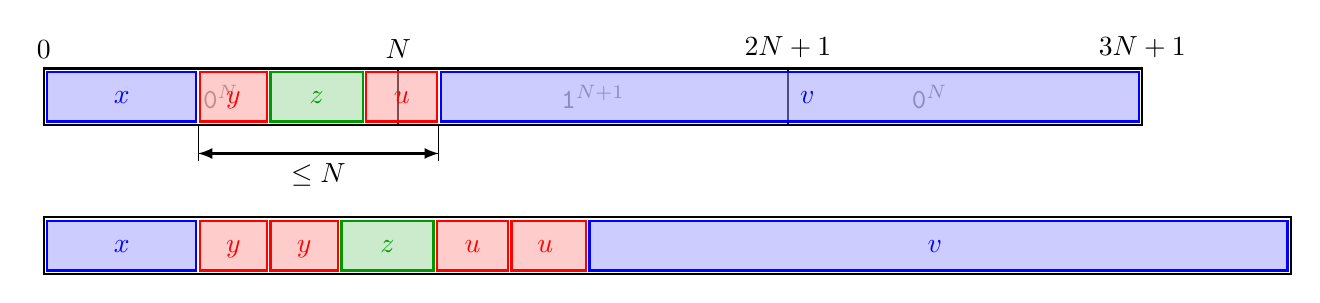
\begin{tikzpicture}[>=latex,thick,scale=0.90]

\draw (0,0) rectangle (5,0.8);
\draw (5,0) rectangle (10.5,0.8);
\draw (10.5,0) rectangle (15.5,0.8);

\node at (0,0.8) [above] {$0$};
\node at (5,0.8) [above] {$N$};
\node at (10.5,0.8) [above] {$2N+1$};
\node at (15.5,0.8) [above] {$3N+1$};

\node[color=gray] at (2.5,0.4) {$\texttt{0}^N$};
\node[color=gray] at (7.75,0.4) {$\texttt{1}^{N+1}$};
\node[color=gray] at (12.5,0.4) {$\texttt{0}^N$};

\fill[color=blue!40,opacity=0.5] (0.05,0.05) rectangle (2.15,0.75);
\draw[color=blue] (0.05,0.05) rectangle (2.15,0.75);
\node[color=blue] at (1.1,0.4) {$x$\strut};

\fill[color=red!40,opacity=0.5] (2.20,0.05) rectangle (3.15,0.75);
\draw[color=red] (2.20,0.05) rectangle (3.15,0.75);
\node[color=red] at (2.675,0.4) {$y$\strut};

\fill[color=darkgreen!40,opacity=0.5] (3.20,0.05) rectangle (4.50,0.75);
\draw[color=darkgreen] (3.20,0.05) rectangle (4.50,0.75);
\node[color=darkgreen] at (3.85,0.4) {$z$\strut};

\fill[color=red!40,opacity=0.5] (4.55,0.05) rectangle (5.55,0.75);
\draw[color=red] (4.55,0.05) rectangle (5.55,0.75);
\node[color=red] at (5.05,0.4) {$u$\strut};

\fill[color=blue!40,opacity=0.5] (5.60,0.05) rectangle (15.45,0.75);
\draw[color=blue] (5.60,0.05) rectangle (15.45,0.75);
\node[color=blue] at (10.775,0.4) {$v$\strut};

\draw[line width=0.3pt] (2.175,0) -- (2.175,-0.5);
\draw[line width=0.3pt] (5.575,0) -- (5.575,-0.5);
\draw[<->] (2.175,-0.4) -- (5.575,-0.4);
\node at (3.875,-0.4) [below] {$\le N$};

\begin{scope}[yshift=-2.1cm]
\draw (0,0) rectangle (17.6,0.8);

\fill[color=blue!40,opacity=0.5] (0.05,0.05) rectangle (2.15,0.75);
\draw[color=blue] (0.05,0.05) rectangle (2.15,0.75);
\node[color=blue] at (1.1,0.4) {$x$\strut};

\fill[color=red!40,opacity=0.5] (2.20,0.05) rectangle (3.15,0.75);
\draw[color=red] (2.20,0.05) rectangle (3.15,0.75);
\node[color=red] at (2.675,0.4) {$y$\strut};

\fill[color=red!40,opacity=0.5] (3.20,0.05) rectangle (4.15,0.75);
\draw[color=red] (3.20,0.05) rectangle (4.15,0.75);
\node[color=red] at (3.675,0.4) {$y$\strut};

\fill[color=darkgreen!40,opacity=0.5] (4.20,0.05) rectangle (5.50,0.75);
\draw[color=darkgreen] (4.20,0.05) rectangle (5.50,0.75);
\node[color=darkgreen] at (4.85,0.4) {$z$\strut};

\fill[color=red!40,opacity=0.5] (5.55,0.05) rectangle (6.55,0.75);
\draw[color=red] (5.55,0.05) rectangle (6.55,0.75);
\node[color=red] at (6.05,0.4) {$u$\strut};

\fill[color=red!40,opacity=0.5] (6.60,0.05) rectangle (7.65,0.75);
\draw[color=red] (6.60,0.05) rectangle (7.65,0.75);
\node[color=red] at (7.075,0.4) {$u$\strut};

\fill[color=blue!40,opacity=0.5] (7.70,0.05) rectangle (17.55,0.75);
\draw[color=blue] (7.70,0.05) rectangle (17.55,0.75);
\node[color=blue] at (12.575,0.4) {$v$\strut};

\end{scope}

\end{tikzpicture}
\end{center}
\item
Da $|yzu|\le N$ kann $yzu$ nur Nullen aus einem der beiden Nullenblöcke
enthalten.
Beim Pumpen nimmt die zahl der Nullen im betroffenen Block zu, jedoch
nicht im anderen, das gempumpte Wort liegt daher nicht mehr in der Sprache.

Es aber noch eine zweite Situation, die beim Pumpen eintreten könnte.
Es könnten in $y$ und $u$ nämlich nur Einsen enthalten sein.
In diesem Fall würde beim Pumpen die Zahl der Einsen zunehmen, was der
Sprachdefinition nicht widerspricht.
Indem man $y$ und $u$ abpumpt, würde aber die Zahl der Einsen von $N+1$
auf einen Wert $\le N$ reduziert, nach Voraussetzung $w\in L$ muss
aber die Anzahl der Einsen $>N$ sein.
Damit tritt auch in diesem Fall ein Widerspruch ein.
\item
Dieser Widerspruch zu der Aussage des Pumping Lemma zeigt, dass die
Annahme, $L$ sei kontextfrei, nicht haltbar ist.
\qedhere
\end{enumerate}
\end{loesung}

\begin{bewertung}
Annahme kontextfrei ({\bf PL}) 1 Punkt,
Pumping Length $N$ ({\bf N}) 1 Punkt,
Wahl eines geeigneten Wortes ({\bf W}) 1 Punkt,
Aufteilung in 5 Teile {(\bf A)} 1 Punkt,
Widerspruch beim Pumpen ({\bf W)} 1 Punkt,
Schlussfolgerung ({\bf S}) 1 Punkt.
\end{bewertung}
